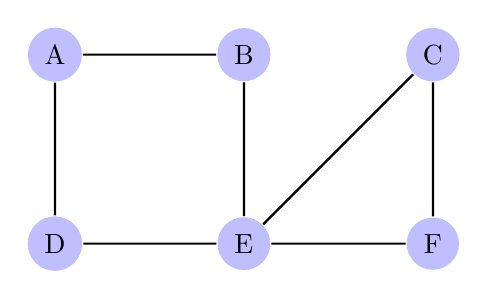
\begin{tikzpicture}
[thick,scale=.8,auto=left,every node/.style={circle,fill=blue!25}]
  \node (n6) at (3,2) {D};
  \node (n4) at (3,5) {A};
  \node (n5) at (6,2) {E};
  \node (n1) at (6,5) {B};
  \node (n2) at (9,2) {F};
  \node (n3) at (9,5) {C};
  \foreach \from/\to in {n6/n4,n5/n1,n2/n5,n2/n3,n1/n4,n6/n5,n5/n3}
    \draw (\from) -- (\to);
\end{tikzpicture}
